\documentclass{beamer}


\usepackage{tabu}
\usepackage[english]{babel}
\usepackage{algorithm}
\usepackage{algpseudocode}

\usepackage[utf8]{inputenc}

\usepackage[english]{babel}
\usepackage{verbatim}
\usepackage{graphicx}
\usepackage{subcaption}
\usepackage{mwe}
\usepackage{amsmath}
\usepackage{bm}
\usepackage{tikz}
\usepackage{verbatim}
\usepackage{textcomp}
\usetikzlibrary{fit, positioning, shapes,arrows}
\usepackage{multirow}
\usepackage{multicol} % Required for multiple columns
\usepackage{algorithm}
\usepackage{algpseudocode}
\usepackage[utf8]{inputenc}
\usepackage[english]{babel}
\usepackage{appendixnumberbeamer}
\DeclareMathOperator{\EX}{\mathbb{E}}% expected value
\usepackage{graphicx}

\usepackage{hyperref}       % hyperlinkssample-bibliography-biblatex
\usepackage{url}            % simple URL typesetting
\usepackage{booktabs}       % professional-quality tables
\usepackage{amsfonts}       % blackboard math symbols
\usepackage{nicefrac}       % compact symbols for 1/2, etc.
\usepackage{microtype}      % microtypography
\usepackage{algorithm}
\usepackage{bm}


\tikzset{three sided/.style={
        draw=none,
        append after command={
            [shorten <= -0.5\pgflinewidth]
            ([shift={(-1.5\pgflinewidth,-0.5\pgflinewidth)}]\tikzlastnode.north east)
        edge([shift={( 0.5\pgflinewidth,-0.5\pgflinewidth)}]\tikzlastnode.north west) 
            ([shift={( 0.5\pgflinewidth,-0.5\pgflinewidth)}]\tikzlastnode.north west)
        edge([shift={( 0.5\pgflinewidth,+0.5\pgflinewidth)}]\tikzlastnode.south west)            
            ([shift={( 0.5\pgflinewidth,+0.5\pgflinewidth)}]\tikzlastnode.south west)
        edge([shift={(-1.0\pgflinewidth,+0.5\pgflinewidth)}]\tikzlastnode.south east)
        }
    }
}

\makeatletter
\DeclareRobustCommand{\rchi}{{\mathpalette\irchi\relax}}
\newcommand{\irchi}[2]{\raisebox{\depth}{$#1\chi$}} 

\newcommand*\bigcdot{\mathpalette\bigcdot@{.5}}
\newcommand*\bigcdot@[2]{\mathbin{\vcenter{\hbox{\scalebox{#2}{$\m@th#1\bullet$}}}}}
\makeatother



% to compile a camera-ready version, add the [final] option, e.g.:
% \usepackage[final]{nips_2016}

\usepackage{nicefrac}       % compact symbols for 1/2, etc.
\usepackage{microtype}      % microtypography
\setbeamerfont{caption}{series=\normalfont,size=\fontsize{6}{6}} 
\usepackage{breakcites}
\usepackage[tableposition=top]{caption}

\usepackage{ragged2e}
\usepackage{etoolbox}
\usepackage{lipsum}


\apptocmd{\frame}{}{\justifying}{} % Allow optional arguments after frame.

\colorlet{Mycolor1}{green!10!orange!90!}
\definecolor{foreground}{RGB}{255,255,255}
\definecolor{background}{RGB}{30,30,30}
\definecolor{title}{RGB}{107,174,214}
\definecolor{gray}{RGB}{155,155,155}
\definecolor{subtitle}{RGB}{102,255,204}
\definecolor{hilight}{RGB}{102,255,204}
\definecolor{vhilight}{RGB}{255,111,207}
\definecolor{footline}{RGB}{255,255,255}

\setbeamercolor{titlelike}{fg=title}
\setbeamercolor{subtitle}{fg=subtitle}
\setbeamercolor{institute}{fg=gray}
\setbeamercolor{normal text}{fg=foreground,bg=background}

\usepackage{lipsum}

\defbeamertemplate{headline}{page number}{%
	\vskip1pt%
	\setbeamertemplate{footline}[page number]%
	\usebeamertemplate{footline}%
}
\setbeamertemplate{headline}[page number]
\setbeamercolor{page number in head/foot}{fg=white}



\usepackage[absolute,overlay]{textpos}

\mode<presentation>
{
  \usetheme{default}      % or try Darmstadt, Madrid, Warsaw, ...
  \usecolortheme{default} % or try albatross, beaver, crane, ...
  \usefonttheme{default}  % or try serif, structurebold, ...
  \setbeamertemplate{navigation symbols}{}
  \setbeamertemplate{caption}[numbered]
} 
\usepackage{acronym}

%%Theo's stuff
\newcommand{\theo}[1]{{\color{blue}Theo: [#1]}}
\newcommand{\edwin}[1]{{\color{green}Edwin: [#1]}}
\newcommand{\virginia}[1]{{\color{red}Virginia: [#1]}}

% abbreviations
\newcommand{\etal}{et al.\xspace}
\newcommand{\ie}{i.e.\xspace}
\newcommand{\eg}{e.g.\xspace}
\newcommand{\Ie}{I.e.\xspace}
\newcommand{\eq}{Eq.\xspace}
\newcommand{\eqs}{Eqs.\xspace}
\newcommand{\fig}{Fig.\xspace}
\newcommand{\secref}[1]{\S \ref{#1}}
\newcommand{\iid}{i.i.d.~\xspace}
\newcommand{\dgp}{DGP\xspace}
\newcommand{\tbl}{Tab.\xspace}


% Acronyms
\newcommand{\supplement}{supplement}
\newcommand{\acro}[1]{\textsc{#1}\xspace}
\newcommand{\lgcp}{\acro{lgcp}}
\newcommand{\icm}{\acro{icm}}
\newcommand{\lgcpn}{\acro{lgcpn}}
\newcommand{\lgcpnnormal}{\acro{lgcpn-n}}
\newcommand{\lgcpngp}{\acro{lgcpn-gp}}
\newcommand{\mlgcp}{\acro{mlgcp}}
\newcommand{\pool}{\acro{pooling}}
\newcommand{\lgcpc}{\acro{lgcp-c}}
\newcommand{\lgcpnc}{\acro{lgcpn-c}}
\newcommand{\gptext}{\acro{gp}}
\newcommand{\mtl}{\acro{mtl}}
\newcommand{\stl}{\acro{stl}}
\newcommand{\mcmc}{\acro{mcmc}}
\newcommand{\mala}{\acro{mala}}
\newcommand{\inla}{\acro{inla}}
\newcommand{\lcm}{\acro{lcm}}
\newcommand{\rbf}{\acro{rbf}}
\newcommand{\btb}{\acro{btb}}
\newcommand{\gt}{\acro{gt}}
\newcommand{\mv}{\acro{mv}}
\newcommand{\nypd}{\acro{nypd}}
\newcommand{\nlpl}{\acro{nlpl}}
\newcommand{\rmse}{\acro{rmse}}
\newcommand{\crime}{\acro{crime}}
\newcommand{\cpu}{\acro{cpu}}
\newcommand{\gb}{\acro{gb}}
\newcommand{\ram}{\acro{ram}}


% Matrices and vectors 
\newcommand{\mat}[1]{\mathbf{#1}}
\renewcommand{\vec}[1]{ \mathbf{#1} } % math bold
\newcommand{\vecS}[1]{\boldsymbol{ #1 }  } % this for boldsymbols
\newcommand{\vecentry}[2]{{\mathrm #1_{#2}}}
\newcommand{\matentry}[3]{{\mathrm #1_{#2,#3}}}
\newcommand{\matcol}[2]{\mat{#1}_{\cdot,#2}}
\newcommand{\matrow}[2]{\mat{#1}_{#2,\cdot}}

% GP things
\newcommand{\gp}{\mathcal{GP}}
\newcommand{\kernel}{\kappa}
\newcommand{\meanfunc}[1]{m(#1)}
\newcommand{\covfunc}[3]{\kernel(#1,#2; #3)}
\newcommand{\hyperparam}{\vectheta}

% Specific variables
\newcommand{\dataset}{\mathcal{D}}
\newcommand{\x}{\vec{x}}
\newcommand{\xn}{\x_n}
\newcommand{\xstar}{\x_\star}
\newcommand{\xprime}{\x^{\prime}}
\newcommand{\vectheta}{\vecS{\theta}}
\newcommand{\y}{\vec{y}}
\newcommand{\ystar}{\y_\star}
\newcommand{\yn}{\vec{y}_n}
\newcommand{\f}{\mat{F}}
\newcommand{\fstar}{\f_\star}
%\newcommand{\u}{\vec{u}}
\newcommand{\fq}{\f_{\bullet q}}
\newcommand{\fn}{\f_{n \bullet}}
\newcommand{\samplefn}[1]{\fn^{(#1)}}
\newcommand{\W}{\mat{W}}
\renewcommand{\wp}{\W_{p \bullet}}
\newcommand{\varw}{\sigma^2} % variance of W for independent prior
\newcommand{\wq}{\W_{\bullet q}}
\newcommand{\samplewp}[1]{\wp^{(#1)}}
\newcommand{\Y}{\mat{Y}}
\newcommand{\lambdan}{\vec{\lambda}_{n \bullet}}
\renewcommand{\u}{\mat{U}}
\newcommand{\uq}{\u_{\bullet q}}
\newcommand{\z}{\vec{z}}
\newcommand{\Z}{\mat{Z}}
\newcommand{\Zq}{\Z_q}
\newcommand{\zprime}{\z^{\prime}}
\newcommand{\meanfu}{\tilde{\vecS{\mu}}}  % conditonal prior mean
\newcommand{\covfu}{\widetilde{\vecS{\mat{K}}}}  % conditonal prior covariance
\newcommand{\meanfuq}{\tilde{\vecS{\mu}}_q}  % conditonal prior mean
\newcommand{\covfuq}{\widetilde{\vecS{\mat{K}}}_q}  % conditonal prior covariance
\newcommand{\likeparam}{\phi}

% Covariance matricces
\newcommand{\Kq}{\mat{K}_{xx}^q}
\newcommand{\covwq}{\vecS{\mat{K}}_{w}^q}
\newcommand{\Kzzq}{\mat{K}_{zz}^q}
\newcommand{\Kxzq}{\mat{K}_{xz}^q}
\newcommand{\Kzxq}{\mat{K}_{zx}^q}
\newcommand{\Kzzqinv}{(\mat{K}_{zz}^q)^{-1}}


% Distributions
\newcommand{\poisson}{\text{Poisson}}
\newcommand{\normal}{\mathcal{N}}

% statistics / algebra / computation
\newcommand{\kl}[2]{\mathrm{KL}(#1 \lVert #2)}
\newcommand{\expectation}[2]{ \mathbb{E}_{#1}{\left[#2\right]} }
\renewcommand{\det}[1]{\left\lvert#1\right\rvert}
\newcommand{\trace}{\mbox{ \rm tr }}
\newcommand{\bigO}{\mathcal{O}}

% variational stuff
\newcommand{\varparam}{\vecS{\nu}}
\newcommand{\varmeanuq}{\vec{m}_q}
\newcommand{\varmeanfqn}{\mu_q}
\newcommand{\varmeanfq}{\pmb{\mu}_q}
\newcommand{\varcovuq}{\mat{S}_q}
\newcommand{\varmeanwq}{\vecS{\omega}_q}
\newcommand{\varmeanwpq}{\omega_{pq}}
\newcommand{\varcovwq}{\vecS{\Omega}_q}
\newcommand{\varcovwpq}{\Omega_{pq}}
\newcommand{\varcovfq}{\Sigma^q}
\newcommand{\varvarwq}{\tilde{\sigma}^2_q}
\newcommand{\calL}{\mathcal{L}}
\newcommand{\elbo}{\calL_{\text{elbo}}}
\newcommand{\ellterm}{\calL_{\text{ell}}}
\newcommand{\klterm}{\calL_{\text{kl}}}
\newcommand{\enterm}{\calL_{\text{ent}}}
\newcommand{\crossterm}{\calL_{\text{cross}}}
\newcommand{\elltermhat}{\widehat{\calL}_{\text{ell}}}  
\newcommand{\qfn}{q(\fn) }
\newcommand{\qwp}{q(\wp)}





\title[]{Fully Bayesian Optimisation}
\author[Juan Ungredda]{\small Juan Ungredda}
\institute[]{University of Warwick}
\date{}


\begin{document}


\begin{frame}
  \titlepage
  \flushright
\includegraphics[ height=0.8cm]{logo_epsrc.jpeg}
  
\includegraphics[ height=0.8cm]{logo_warwick.jpeg}
\end{frame}

\begin{frame}{Outline}
	Background \& Motivation\\
	\vspace{5mm}
	Including Input Uncertainty over Hyperparameters
	\begin{itemize}
		\item Impact on Bayesian Optimisation
		\item Results
		\item Several (Markov Chain Monte Carlo) MCMC approximations
	\end{itemize}
\end{frame}

\section{Background}

\begin{frame}{Background: Gaussian Process Approximation}
magenta
Given a random variable that represents the value of the function $f(\mathbf{x})$ at location $\mathbf{x}$. A Gaussian process is a collection of random variables, any finite number of which have a joint Gaussian distribution.

\begin{align*}
\begin{split}
m(x) &= \mathbb{E}[f(\mathbf{x})]\\
k_{\theta}(\mathbf{x},\mathbf{x}') &=\mathbb{E}[(f(\mathbf{x}) - m(x))(f(\mathbf{x'}) - m(x'))]
\end{split}
\end{align*}

Usually, $m(x) = \mathbf{0}$ as prior with a user-defined kernel $k(\mathbf{x},\mathbf{x}')$.
\end{frame}

\begin{frame}{Background: Kernels}

$k(\mathbf{x},\mathbf{x}')$ imposes stronger preferences for certain types of functions, i.e. smooth or stationary functions, or functions with certain lengthscales.
\vspace{3mm}

Common choices of kernels $k_{\theta}(\mathbf{x},\mathbf{x}') $.\\
\begin{itemize}
	\item Square Exponential: $\sigma^{2}_{f}exp\{-\frac{1}{2}(\mathbf{x}-\mathbf{x'})^{T}\Sigma^{-1}(\mathbf{x}-\mathbf{x'})\}$
	\item Matern 5/2 Kernel: $\alpha(1+\sqrt{5}r+\frac{5}{3}r^{2})exp\{-\sqrt{5}r\}$; where $r=\frac{||\mathbf{x} - \mathbf{x'}||_{2}}{l}$
\end{itemize}
\end{frame}

\begin{frame}{Background: Prediction}
Consider the possible designs $x \in X$, and a function $f$: $X \rightarrow \mathbb{R}$.\\
$$y(x) = f(x) +\epsilon,\text{ where }\epsilon \sim N(0,\sigma^{2}_{\epsilon})$$

The posterior distribution of latent variables is\footnote{$f^{*}$ is the result of evaluating $f(x)$ at new design $x^{*}$}

$$ p(f,f^{*}|y,\theta) = \frac{ \textcolor{green}{\overbrace{p(y|f)}^{Likelihood}}\textcolor{yellow}{\overbrace{p(f,f^{*}|\theta)}^{prior}}}{ \textcolor{magenta}{\underbrace{p(y|\theta)}_{Marginal Likelihood}}} $$

\end{frame}

\begin{frame}{Background: Prediction}

The posterior predictive distribution is,\footnote{Simplified notation:  $k_{\theta}(\mathbf{x},\mathbf{x'}) = k_{f,f}$ and $k_{y,y} = k_{f,f} + \sigma^{2}_{\epsilon}$}

$$p(f^{*}|y,\theta)  \propto \int \textcolor{green}{\underbrace{p(y|f)}_\text{Likelihood}} \textcolor{yellow}{\underbrace{p(f,f^{*}|\theta)}_\text{Prior}} df$$

Commonly, \textcolor{green}{$p(y|f) \sim N(y; f , \sigma^{2}_{\epsilon})$} and \textcolor{yellow}{$p(f,f^{*}|\theta) \sim N(f,f^{*}; \mathbf{0} , k_{\theta}(\mathbf{x},\mathbf{x'}))$}


\begin{align*}
\begin{split}
p(f^{*}|y,\theta) &= N(\mu^{n},\Sigma^{n}) \text{, where} 
\end{split}\\
\begin{split}
\mu^{n} &= k_{*,f}k^{-1}_{y,y}y
\end{split}\\
\begin{split}
\Sigma^{n} &= k_{*,*} - k_{*,f}k_{y,y}^{-1}k_{f,*}
\end{split}
\end{align*}

\end{frame}
\begin{frame}{Background: Point Estimation for Hyperparameters}

\begin{itemize}
	\item Maximum Likelihood (ML):
	\begin{align*}
	\begin{split}
	\hat{\theta}= arg \max_{\theta \in \Theta} \{log(\textcolor{magenta}{p(y|\theta)}) \}
	\end{split}
	\end{align*}
	
	\item Maximum a Posteriori (MAP):
	\begin{align*}
	\begin{split}
	E &= log(p(\theta|y)) = log(p(y|\theta)) + log(p(\theta))
	\end{split}\\
	\begin{split}
	\hat{\theta} &= arg \max_{\theta \in \Theta}\{E\}  
	\end{split}
	\end{align*}
\end{itemize}


\end{frame}

\begin{frame}{Motivation}
Potential issues of point estimations,

\begin{itemize}
	\item Multimodality
	\item Deceptive functions
	\item Uncertainty Underestimation
\end{itemize}

\end{frame}

\begin{frame}{Motivation: Multimodality}

\begin{itemize}
	\item Likelihood may be multimodal. Solutions may converge to poor local maxima. 	
	\begin{figure}
		\centering
		\begin{tabular}{c}
			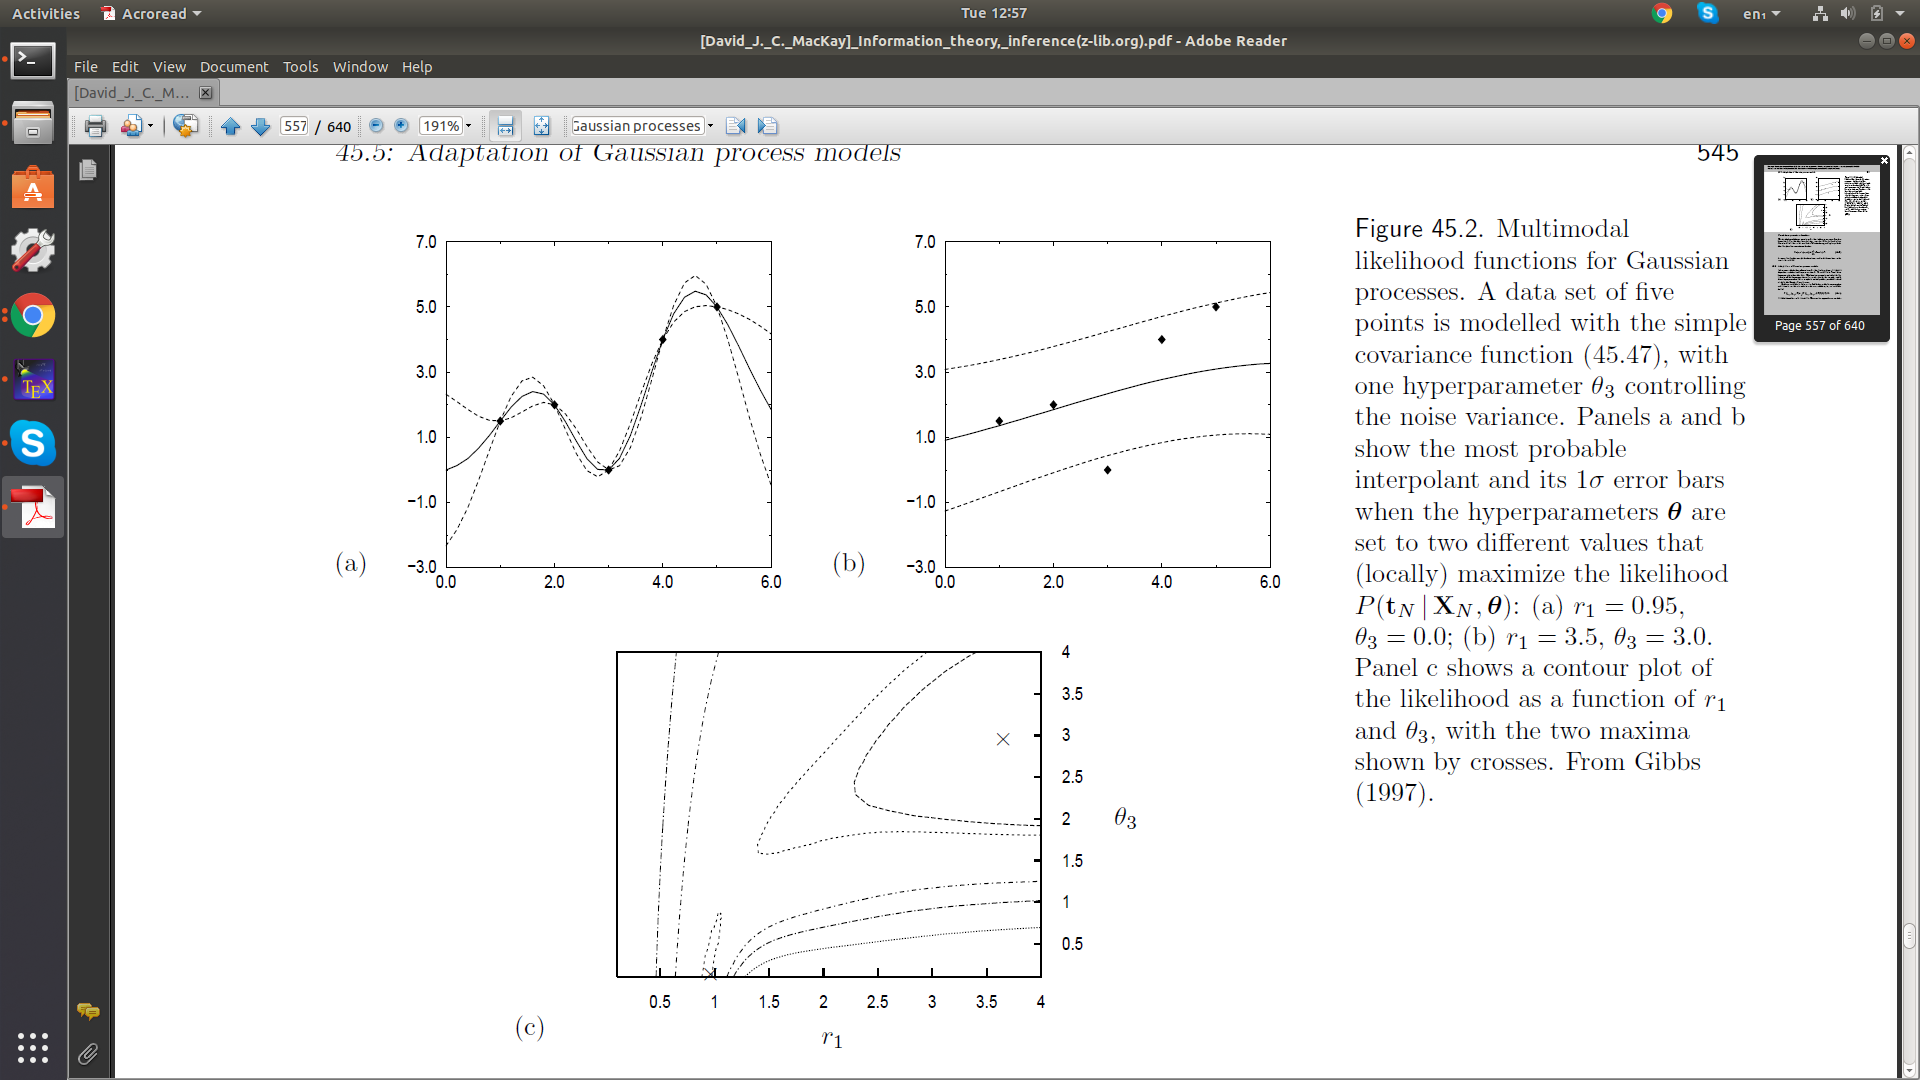
\includegraphics[width=8cm, trim={11.5cm 1cm 20cm 7cm},clip]{Mackay.png}
		\end{tabular}
	\captionof{figure}{MacKay, D. (2002) "\textit{Information Theory, Inference \& Learning Algorithms}"}
	\end{figure}
\end{itemize}

\end{frame}

\begin{frame}{Motivation: Deceptive functions}

\begin{itemize}
	\item \textit{Deceptive functions}: Describe functions that appear to be “flat” based on evaluation results.
		
	\begin{figure}
		\centering
		\begin{tabular}{c}
			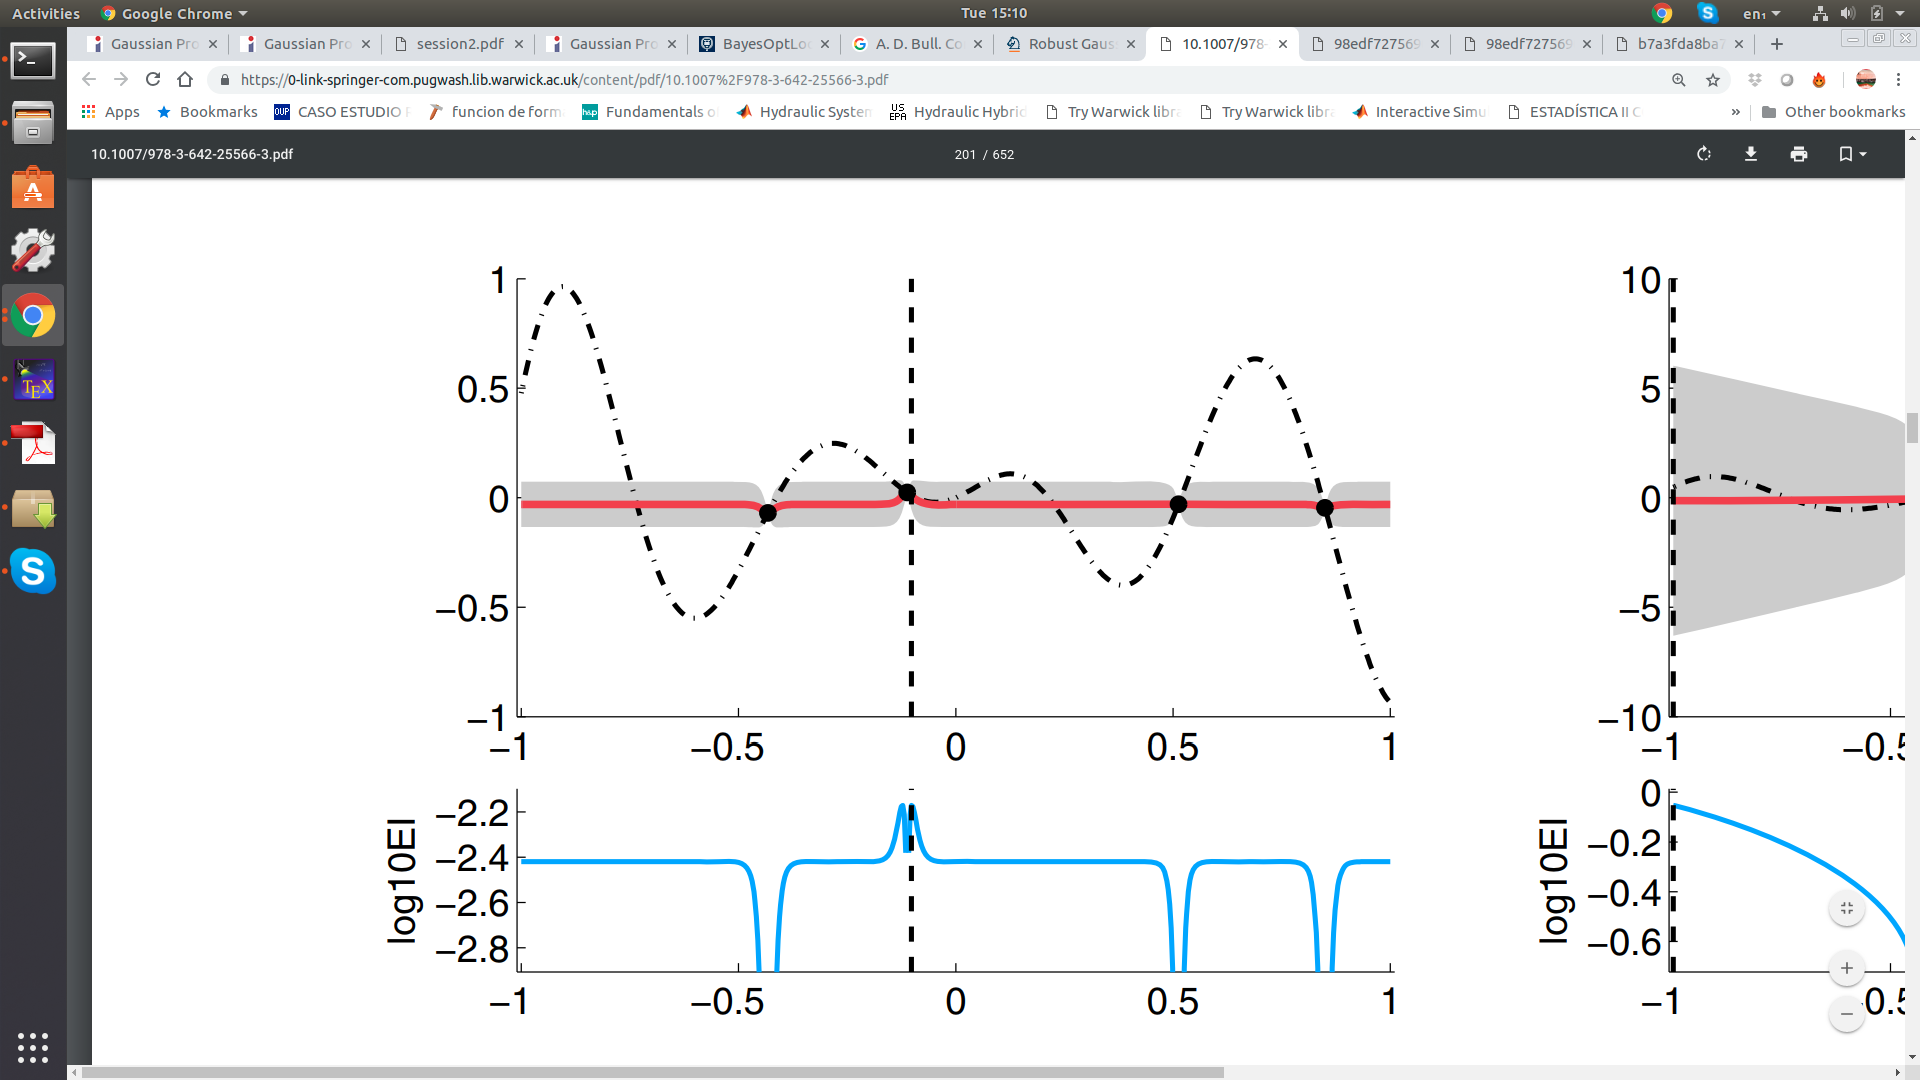
\includegraphics[width=8cm, trim={11.5cm 1cm 16cm 7cm},clip]{Decep_Func.png}
		\end{tabular}
		\captionof{figure}{Benassi R., et al.(2011)}
	\end{figure}

\end{itemize}
\end{frame}




\begin{frame}{Motivation: Uncertainty Underestimation}

\begin{itemize}
	\item  Standard deviation of the error of prediction is underestimated. 
	
	\begin{figure}
		\centering
		\begin{tabular}{c}
			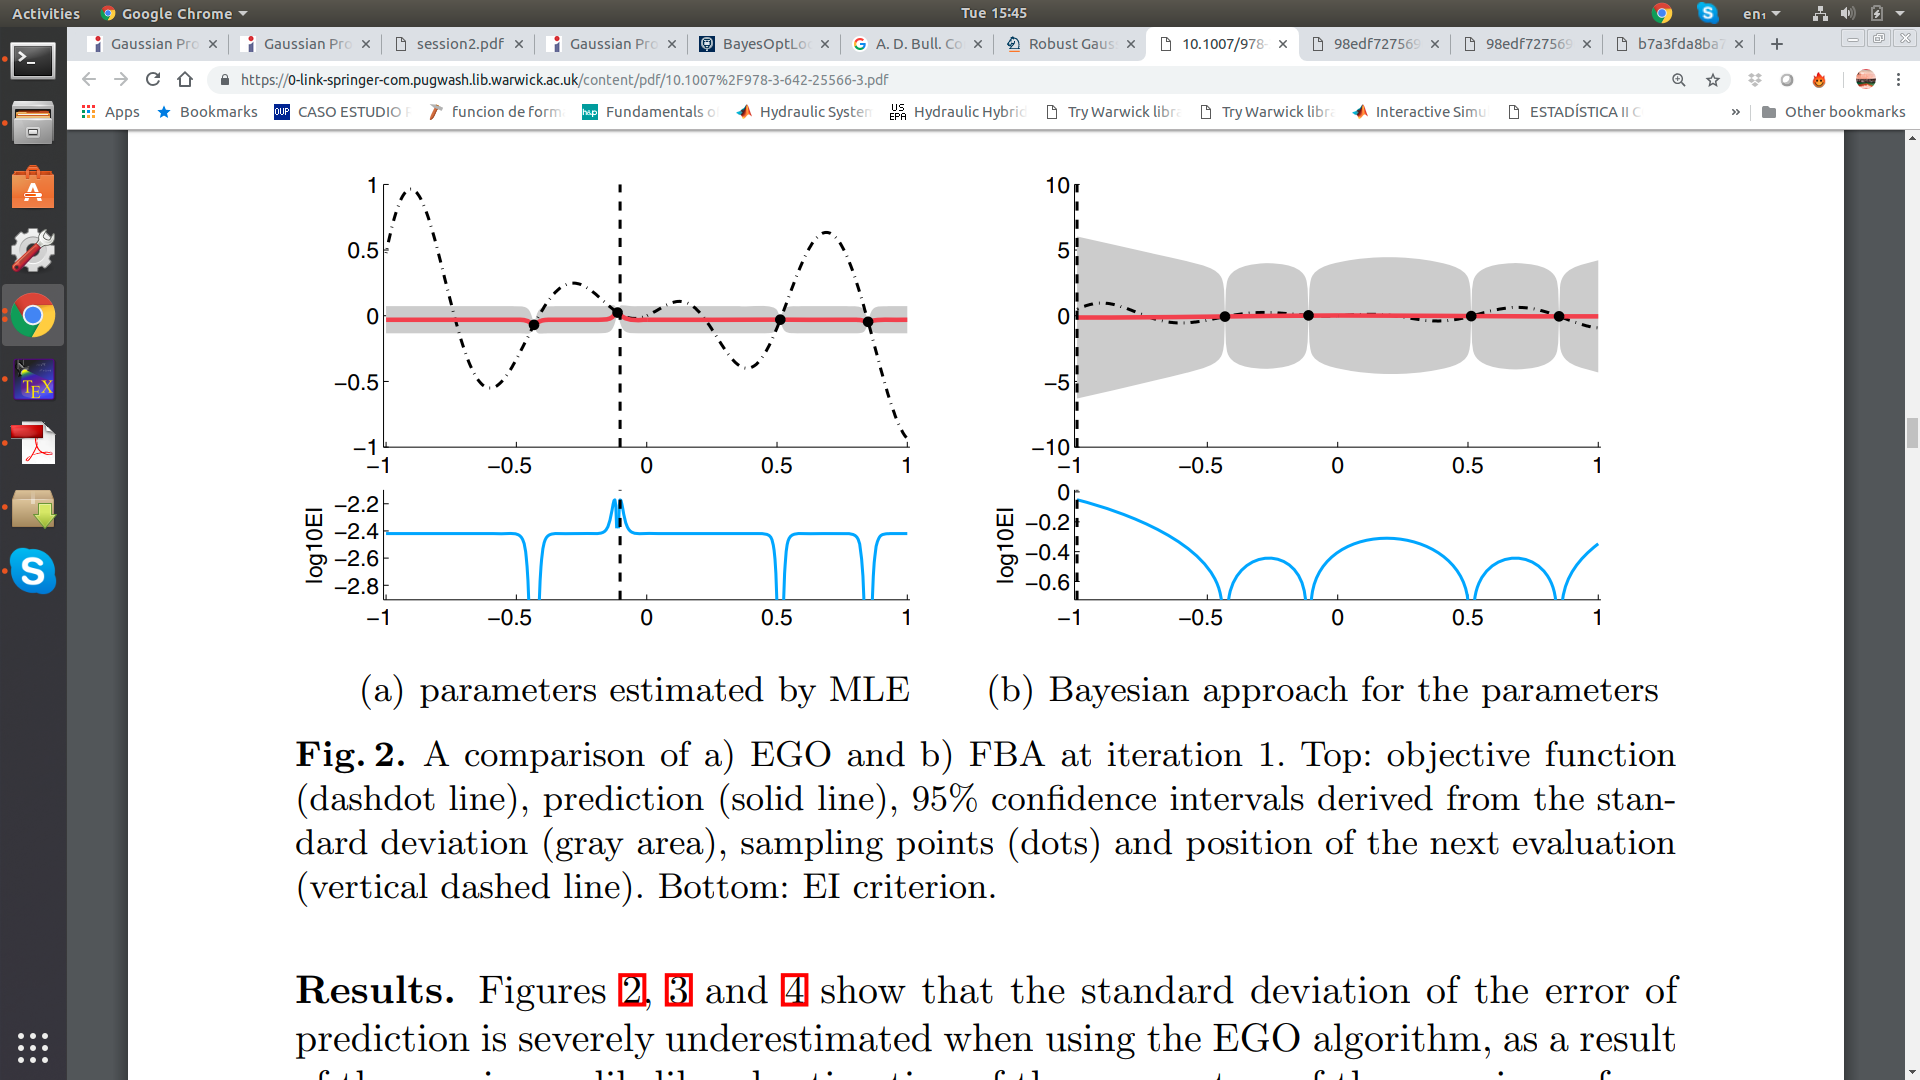
\includegraphics[width=9cm, trim={11.5cm 13cm 7.5cm 6cm},clip]{decep_func_conf.png}
		\end{tabular}
		\captionof{figure}{Benassi R., et al.(2011)}
	\end{figure}
	
\end{itemize}

\end{frame}

\begin{frame}{Including Input Uncertainty over Hyperparameters}
\begin{figure}
	\centering
	\begin{tabular}{c}
		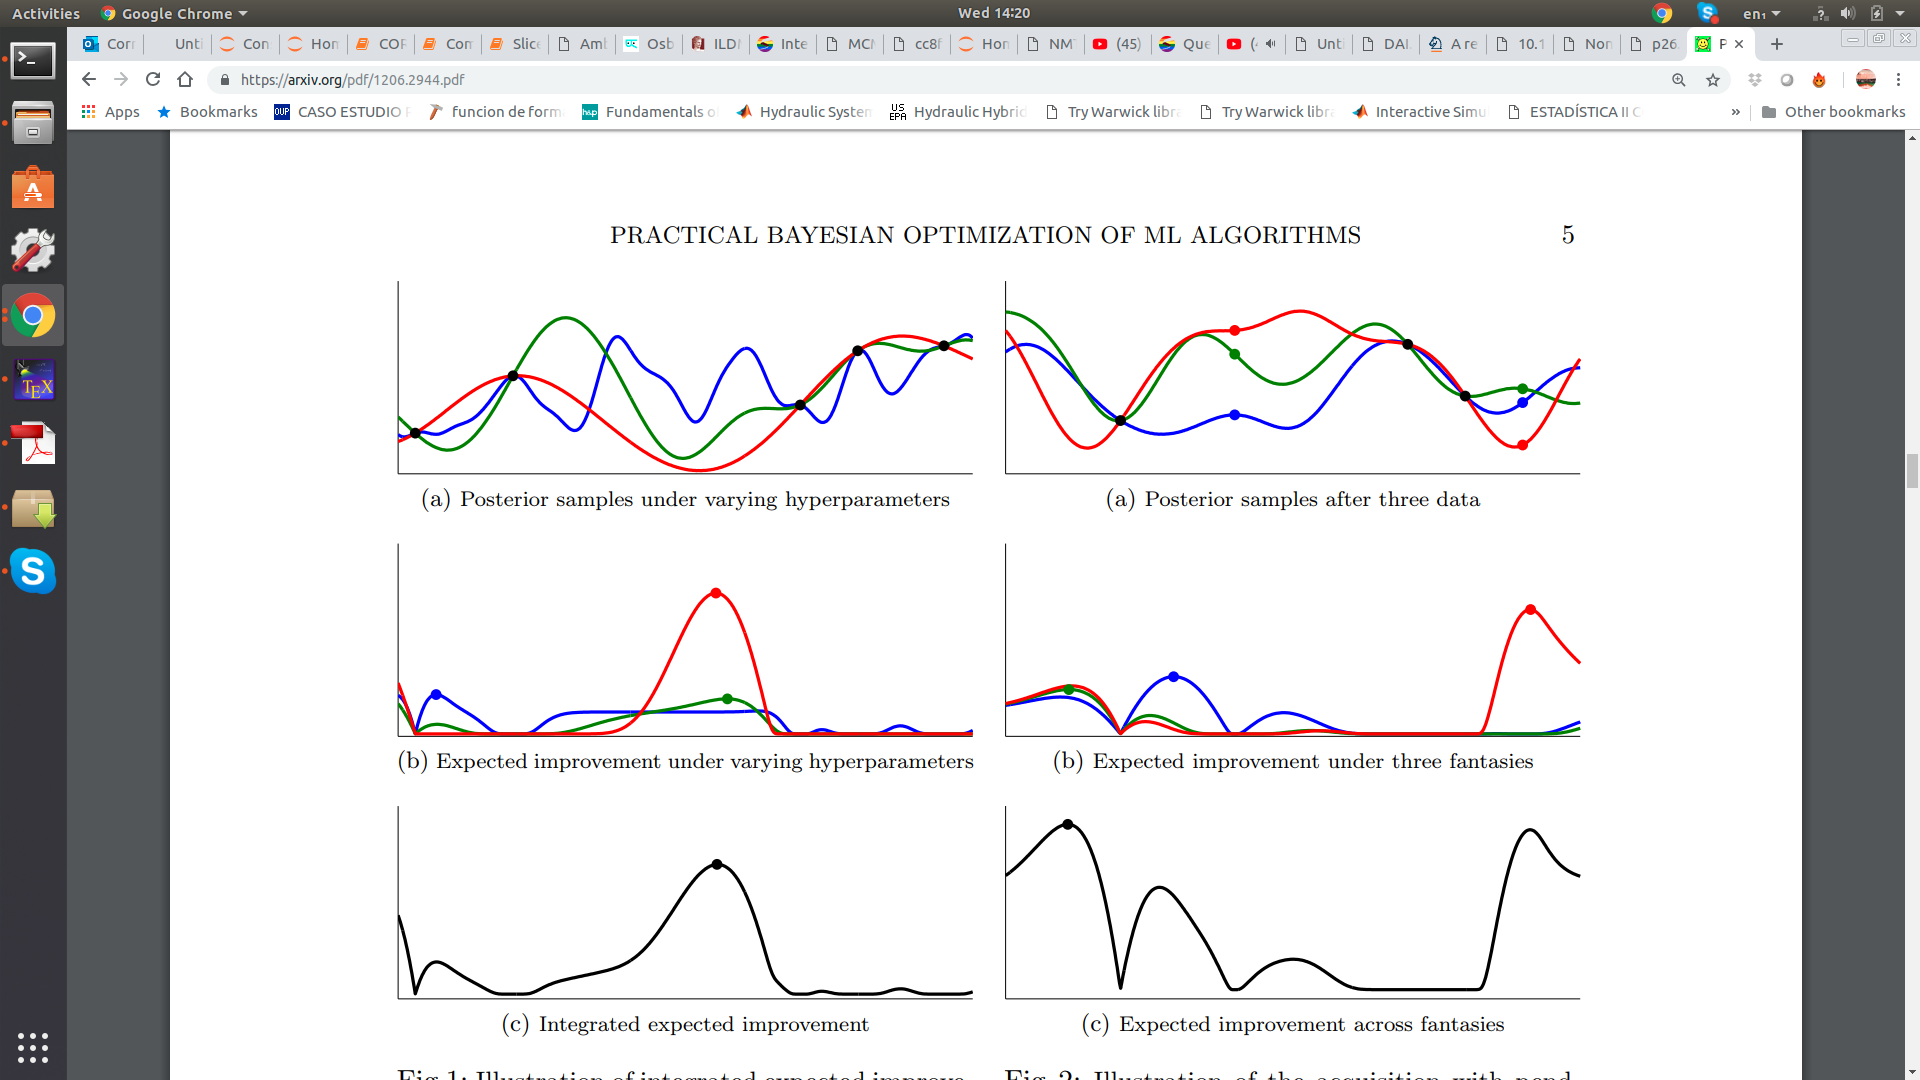
\includegraphics[width=5cm, trim={11.5cm 1cm 33cm 9cm},clip]{dif_hyp_params.png}
	\end{tabular}
	\captionof{figure}{Snoek J., et al.(2012)}
\end{figure}
\end{frame}

\begin{frame}{Impact on Bayesian Optimisation}

Strategies for Optimisation:\\
\begin{itemize}
	\item $EI(x)_{\theta^{ML}}$: Use ML estimates for Expected Improvement.
	\item $EI(x)_{\theta^{True}}$: Use True Hyperparameters.
	\item $\mathbb{E}_{\theta}[EI(x)]$: Marginalising Hyperparameters.
\end{itemize}

Performance metric:\\
\vspace{3mm}
$Opportunity\text{ }Cost(OC) = \max\{f(x)\} - \max_{i=1,\dots,n}\{y_{i}\}$

where,
\begin{itemize}
	\item $f(x)$ = True function
	\item $y_{i}$ = sampled data
\end{itemize}

\end{frame}

\begin{frame}{Results}
content...
\end{frame}

\begin{frame}{MCMC approximations}
\begin{center}
	\begin{tabu} to 1.0 \textwidth{||X[l] X[c]||} 
		\hline
		Algrthm & Parameters\\ [0.5ex] 
		\hline\hline
		Hamiltonian Monte Carlo \newline {\scriptsize(Y. Saatc, et al.(2010))} & Leapfrog steps \newline Leapfrog $\Delta t$  \\ 
		\hline
		Slice Sampling\newline {\scriptsize(Murray, et al.(2010))} & noise level $S_{\theta}$  \\
		\hline
		Sequential Monte Carlo \newline {\scriptsize(A. Svensson, et al. (2015))} & Partition P \newline MH-moves K \newline Proposal distribution q  \\
		\hline
		 Bayesian
		Monte Carlo \newline {\scriptsize(Osborne M. A., et al (2008))}  & Hyperparameters of GP Approximation \\
		\hline
		 Adaptive Importance Sampling \newline {\scriptsize(Petelin D., et al (2014))} & Proposal distribution  q\\ [1ex] 
		\hline
	\end{tabu}
\end{center}
\end{frame}



\begin{frame}{References}
\begin{itemize}
	
	{\scriptsize
	\item Benassi R., Bect J., Vazquez E. (2011) "Robust Gaussian Process-Based Global Optimization Using a Fully Bayesian Expected Improvement Criterion. In: Coello C.A.C. (eds) Learning and Intelligent Optimization". LION 2011. Lecture Notes in Computer Science, vol 6683. Springer, Berlin, Heidelberg
	
	\item M. A. Osborne, S. J. Roberts, A. Rogers, S. D. Ramchurn, and N. R.
	Jennings, “Towards real-time information processing of sensor network
	data using computationally efficient multi-output Gaussian processes,”
	in Proceedings of the 7th international conference on information
	processing in sensor networks, St. Louis, MO, USA, Apr. 2008, pp.
	109–120.
	
	\item Murray, Iain and Adams, Ryan Prescott,"Slice sampling covariance hyperparameters of latent Gaussian models" Proceedings of the 23rd International Conference on Neural Information Processing Systems - Volume 2, 2010.
	
	\item Y. Saatc i, R. D. Turner, and C. E. Rasmussen, “Gaussian process change
	point models,” in Proceedings of the 27th International Conference on
	Machine Learning (ICML), Haifa, Israel, Jun. 2010, pp. 927–934.
	
	\item  D. Petelin, M. Gasperin, and V.  Smidl, “Adaptive importance sampling
	for Bayesian inference in Gaussian process models,” in Proceedings of
	the 19th IFAC World Congress, Cape Town, South Africa, Aug. 2014,
	pp. 5011–5015.
}
	
\end{itemize}
\end{frame}

\begin{frame}{References}
\begin{itemize}
	
	{\scriptsize
		\item A. Svensson, J. Dahlin and T. B. Schön, "Marginalizing Gaussian process hyperparameters using sequential Monte Carlo," 2015 IEEE 6th International Workshop on Computational Advances in Multi-Sensor Adaptive Processing (CAMSAP), Cancun, 2015, pp. 477-480.
		
		\item Jasper Snoek, Hugo Larochelle, and Ryan P. Adams. 2012. Practical Bayesian optimization of machine learning algorithms. In Proceedings of the 25th International Conference on Neural Information Processing Systems - Volume 2 (NIPS'12), F. Pereira, C. J. C. Burges, L. Bottou, and K. Q. Weinberger (Eds.), Vol. 2. Curran Associates Inc., USA, 2951-2959.
		
		
	}
	
\end{itemize}
\end{frame}



\end{document}